% Nallino, Part II p. 248: the latitude of a superior planet, redrawn from the print at the size of the print. The
% coordinates are those of a 400 dpi render of the figure (crop from x 120 pt, y 175 pt of the master page;
% y downward). The epicycle ZDGA has its centre in H; GZ and DA are diameters, HE the line to the Earth E; T is the
% planet, K the foot of its perpendicular on DA, L and B the feet of the perpendiculars from T and K on the plane of
% the ecliptic, N the foot of the perpendicular from K on EH. Dashed as on the print: TH, TL, TK, TE, KB, KN, KE, LB
% and LE.
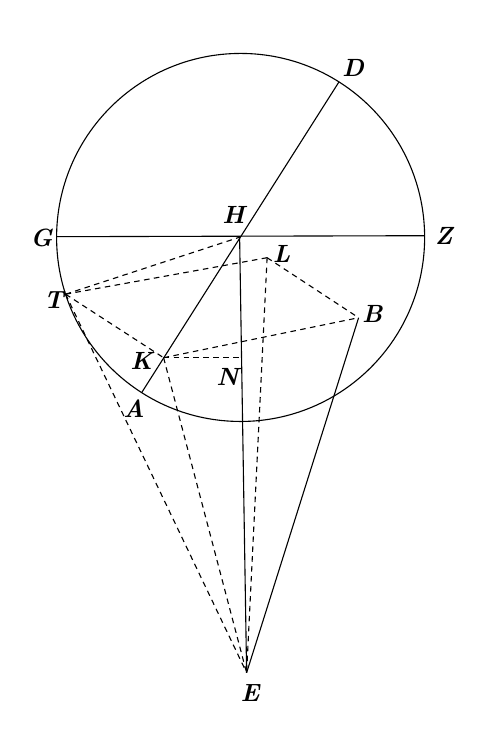
\begin{tikzpicture}[x=0.0635mm,y=-0.0635mm,line width=0.4pt,every node/.style={font=\bfseries\itshape\small,inner sep=1pt}]
\path (300,-50);
\coordinate (H) at (386,369);
\coordinate (E) at (400,1240);
\coordinate (D) at (585,58);
\coordinate (A) at (190,680);
\coordinate (T) at (38,483);
\coordinate (K) at (234,610);
\coordinate (L) at (441,410);
\coordinate (B) at (624,530);
\coordinate (N) at (389,610);
\draw (388,369.5) circle[radius=368];
\draw (20,368) -- (756,366);
\draw (D) -- (A);
\draw (H) -- (E);
\draw (B) -- (E);
\begin{scope}[dash pattern=on 2pt off 1.6pt]
\draw (T) -- (H);
\draw (T) -- (L);
\draw (T) -- (K);
\draw (T) -- (E);
\draw (K) -- (B);
\draw (K) -- (N);
\draw (K) -- (E);
\draw (L) -- (B);
\draw (L) -- (E);
\end{scope}
\node at (613,31) {D};
\node at (-10,370) {G};
\node at (374,325) {H};
\node at (794,367) {Z};
\node at (470,403) {L};
\node at (14.5,494.5) {T};
\node at (651.5,523.5) {B};
\node at (190,617) {K};
\node at (362,649) {N};
\node at (174.5,712.5) {A};
\node at (407,1281) {E};
\end{tikzpicture}
